\chapter[Nonlinear Structure and Reionization]{Nonlinear Structure, Halo Formation, and Reionization Consistency}
\PhysicsContext{From linear transport to structure}{The fourth part tests whether the linear cutoff survives nonlinear gravity and astrophysical response. Several initially strong linear signatures are weakened or rendered sign-indefinite by this progression.}


\label{ch:nonlinear-structure-halo}

\section{Scope and objective}

The scale-covariant refinement sector now supplies a linear collisionless transfer, primary-CMB templates, reionization, and CMB lensing.  The remaining major structure-formation question is whether the linear small-scale cutoff survives nonlinear collapse, and whether the same cutoff is compatible with the early halo population needed by the calibrated reionization history.

This chapter performs a controlled nonlinear consistency audit.  It combines the fixed collisionless transfer with a spherical-collapse calculation, an excursion-set halo abundance, a formation-time concentration model, a compensated halo model, nonlinear lensing projection, and an atomic-cooling collapsed-fraction test.  No dark-sector parameter is retuned.

The principal conclusion is mixed and therefore important:
\begin{equation}
 \boxed{
 \begin{gathered}
 \text{low-mass halo abundance and high-redshift collapse remain strongly suppressed},\\
 \text{but nonlinear halo formation regenerates much of the small-scale power}. 
 \end{gathered}}
 \label{eq:nlh-central-result}
\end{equation}
Consequently, the earlier linear high-$\ell$ galaxy-lensing deficit is not a robust final prediction once a controlled nonlinear halo model is inserted.  The cleaner surviving signatures are the low-mass halo mass function, delayed halo formation, reduced concentrations, and the ionizing-efficiency burden at high redshift.

\section{Fixed linear input and variance ordering}

Let the cold-control spectrum be
\begin{equation}
 P_{\rm c}(k,z)=D(z)^2P_{\rm c}(k,0),
 \label{eq:nlh-cold-power}
\end{equation}
and let the refinement spectrum be
\begin{equation}
 P_D(k,z)=T_D(k)^2P_{\rm c}(k,z),
 \qquad
 0\leq T_D(k)\leq1.
 \label{eq:nlh-dark-power}
\end{equation}
The amplitude is normalized by
\begin{equation}
 \sigma_8=0.81.
 \label{eq:nlh-sigma8}
\end{equation}
For a spherical top-hat containing mass $M$,
\begin{equation}
 R(M)=\left(\frac{3M}{4\pi\bar\rho_m}\right)^{1/3},
 \label{eq:nlh-radius}
\end{equation}
and
\begin{equation}
 \sigma_X^2(M,z)
 =\int_0^\infty
 \frac{k^3P_X(k,z)}{2\pi^2}
 W_{\rm TH}(kR)^2\,d\log k,
 \qquad
 X\in\{\mathrm c,D\}.
 \label{eq:nlh-variance}
\end{equation}
Because the kernel is nonnegative,
\begin{equation}
 \boxed{
 \sigma_D^2(M,z)\leq\sigma_{\rm c}^2(M,z)
 }
 \label{eq:nlh-variance-ordering}
\end{equation}
for every mass and redshift in the declared linear model.  Hence the peak height
\begin{equation}
 \nu_X(M,z)=\frac{\delta_c(z)}{\sigma_X(M,z)}
 \label{eq:nlh-peak-height}
\end{equation}
satisfies
\begin{equation}
 \nu_D(M,z)\geq\nu_{\rm c}(M,z).
 \label{eq:nlh-peak-order}
\end{equation}
This establishes delayed collapse before any halo-mass-function prescription is chosen.

The transfer half-mode is defined by
\begin{equation}
 T_D(k_{1/2})^2=\frac12.
 \label{eq:nlh-half-mode}
\end{equation}
The fixed collisionless transfer gives
\begin{equation}
 \boxed{
 k_{1/2}=7.3571107374\ {\rm Mpc}^{-1}
 }
 \label{eq:nlh-half-mode-value}
\end{equation}
and the associated Lagrangian mass is
\begin{equation}
 \boxed{
 M_{1/2}
 =\frac{4\pi}{3}\bar\rho_m
 \left(\frac{\pi}{k_{1/2}}\right)^3
 =1.3749738169\times10^{10}\ M_\odot.
 }
 \label{eq:nlh-half-mode-mass}
\end{equation}

\begin{figure}[htbp]
\centering
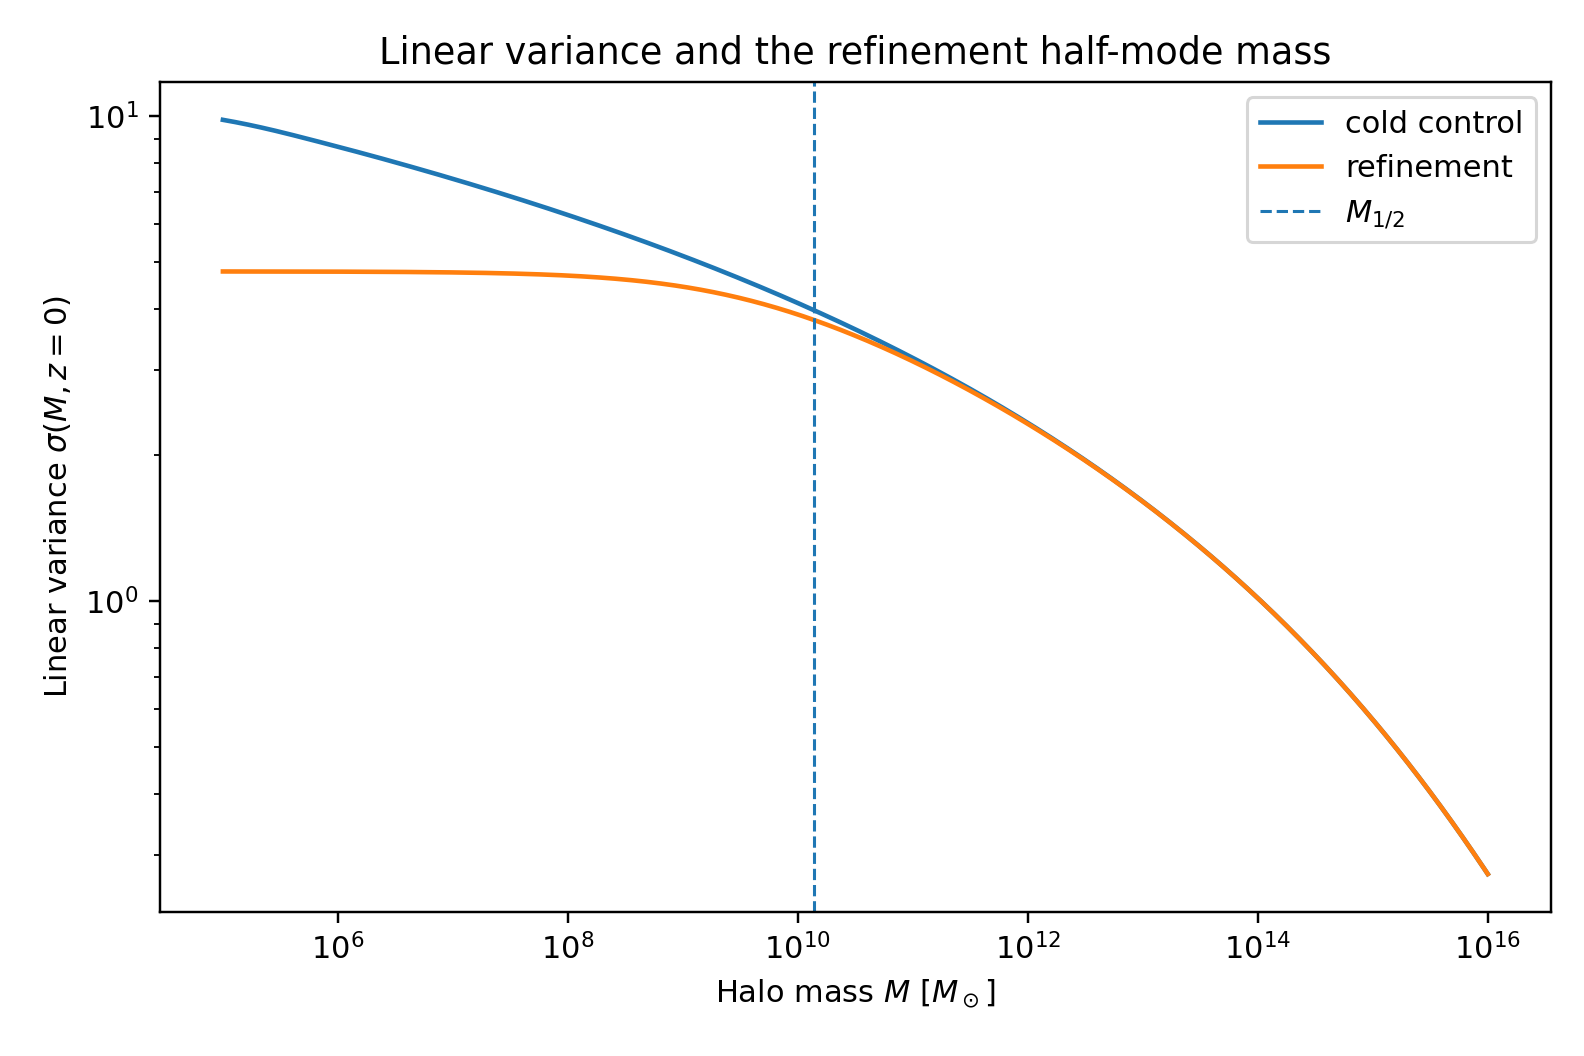
\includegraphics[width=0.86\textwidth]{figures/nls/variance_half_mode.png}
\caption{The linear variance of the cold control and the refinement model.  The ordering is exact within the declared linear spectrum.  The vertical line marks the power half-mode mass.}
\label{fig:nlh-variance}
\end{figure}

\section{Spherical-collapse threshold}

The nonlinear top-hat contrast obeys
\begin{equation}
 \delta''
 +\left(2+\frac{d\log H}{d\log a}\right)\delta'
 -\frac{4}{3}\frac{\delta'^2}{1+\delta}
 -\frac{3}{2}\Omega_m(a)\delta(1+\delta)=0,
 \label{eq:nlh-spherical-collapse}
\end{equation}
where a prime denotes $d/d\log a$.  The initial amplitude is tuned so that the nonlinear solution reaches a declared collapse threshold at the target redshift.  The same initial data are then evolved through the linearized equation, defining $\delta_c(z)$.

The deterministic calculation gives
\begin{equation}
 \delta_c(0)=1.6761139702,
 \qquad
 \delta_c(1)=1.6850426394,
 \qquad
 \delta_c(2)=1.6869970517.
 \label{eq:nlh-delta-c-values}
\end{equation}
The threshold is common to both dark-matter models because their late-time gravitational collapse law is the same.  Their difference enters through $\sigma(M,z)$ and therefore through the abundance of initial peaks.

\section{Excursion-set halo abundance}

The controlled abundance model uses
\begin{equation}
 \frac{dn}{d\log M}
 =\frac{\bar\rho_m}{M}
 f(\nu)
 \left|\frac{d\log\nu}{d\log M}\right|,
 \label{eq:nlh-mass-function}
\end{equation}
with
\begin{equation}
 f(\nu)
 =A_{\rm ST}
 \sqrt{\frac{2a_{\rm ST}}{\pi}}
 \left[1+(a_{\rm ST}\nu^2)^{-p_{\rm ST}}\right]
 \nu e^{-a_{\rm ST}\nu^2/2},
 \label{eq:nlh-st-function}
\end{equation}
where
\begin{equation}
 A_{\rm ST}=0.3222,
 \qquad
 a_{\rm ST}=0.707,
 \qquad
 p_{\rm ST}=0.3.
 \label{eq:nlh-st-parameters}
\end{equation}
These coefficients are a controlled halo-model input, not a derivation from the projector action.

At $z=0$, the refinement-to-cold halo-abundance ratios are
\begin{equation}
 \begin{array}{c|ccccccc}
 M/M_\odot
 &10^7&10^8&10^9&10^{10}&10^{11}&10^{12}&10^{13}\\
 \hline
 (dn/d\log M)_D/(dn/d\log M)_{\rm c}
 &0.0541&0.1746&0.4464&0.7662&0.9335&0.9840&0.9961.
 \end{array}
 \label{eq:nlh-mass-ratios-z0}
\end{equation}
At $z=8$, the corresponding ratios at $10^8$, $10^9$, and $10^{10}M_\odot$ are
\begin{equation}
 \boxed{
 0.0690,
 \qquad
 0.2442,
 \qquad
 0.5544.
 }
 \label{eq:nlh-mass-ratios-z8}
\end{equation}
Thus the cutoff primarily removes low-mass, early-forming halos while leaving cluster-scale abundance nearly unchanged.

\begin{figure}[htbp]
\centering
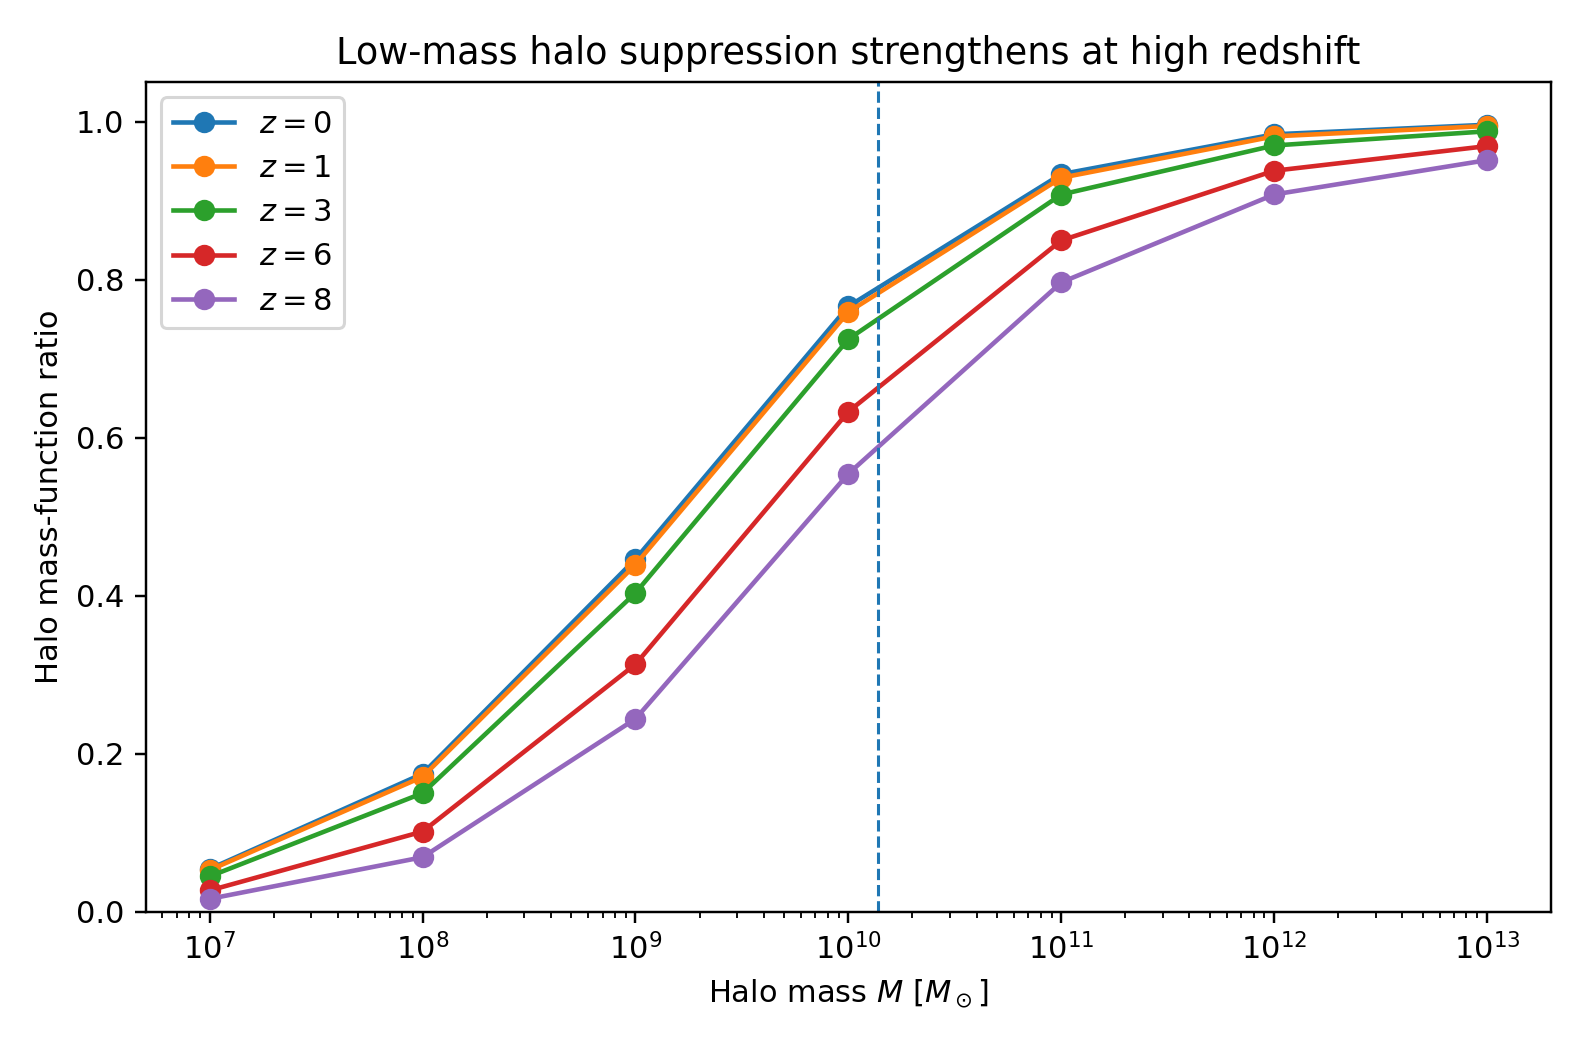
\includegraphics[width=0.86\textwidth]{figures/nls/halo_mass_function_ratios.png}
\caption{Refinement-to-cold halo-abundance ratios in the controlled excursion-set calculation.  The suppression is strongest below the half-mode mass and strengthens toward high redshift.}
\label{fig:nlh-mass-function}
\end{figure}

\section{Formation delay and concentration suppression}

A controlled formation epoch is defined by
\begin{equation}
 D(z_f)\sigma(FM,0)=\delta_{c,\rm EdS},
 \qquad
 F=0.04.
 \label{eq:nlh-formation-redshift}
\end{equation}
The concentration model is
\begin{equation}
 c(M,z)=4\frac{1+z_f}{1+z}.
 \label{eq:nlh-concentration}
\end{equation}
This is used only to propagate the formation delay into a halo-profile template.

At $z=0$,
\begin{equation}
 \begin{array}{c|ccc}
 M/M_\odot
 &10^8&10^{10}&10^{12}\\
 \hline
 z_{f,\rm c}&4.9763&3.2020&1.6202\\
 z_{f,D}&2.5809&2.4305&1.5464\\
 c_D/c_{\rm c}&0.5992&0.8164&0.9718.
 \end{array}
 \label{eq:nlh-concentration-table}
\end{equation}
The refinement cutoff therefore predicts later formation and lower concentrations primarily in low-mass halos.

\section{Compensated nonlinear halo model}

For an NFW profile with normalized Fourier transform $u(k|M)$, define the Lagrangian top-hat window $W(kR_L)$.  The compensated one-halo term is
\begin{equation}
 P_{1h}(k)
 =\int d\log M\,
 \frac{dn}{d\log M}
 \left(\frac{M}{\bar\rho_m}\right)^2
 \left[u(k|M)-W(kR_L)\right]^2.
 \label{eq:nlh-one-halo}
\end{equation}
The subtraction enforces
\begin{equation}
 P_{1h}(k)=O(k^4)
 \label{eq:nlh-one-halo-k4}
\end{equation}
at low wavenumber.  The measured slope is
\begin{equation}
 \boxed{p_{1h}=3.9978690925.}
 \label{eq:nlh-one-halo-slope}
\end{equation}

The normalized two-halo term is
\begin{equation}
 P_{2h}(k)
 =P_{\rm lin}(k)
 \left[
 \frac{
 \int d\log M\,(dn/d\log M)b(M)(M/\bar\rho_m)u(k|M)
 }{
 \int d\log M\,(dn/d\log M)b(M)(M/\bar\rho_m)
 }
 \right]^2.
 \label{eq:nlh-two-halo}
\end{equation}
The total template is
\begin{equation}
 P_{\rm nl}=P_{1h}+P_{2h}.
 \label{eq:nlh-total-power}
\end{equation}

The resulting refinement-to-cold nonlinear ratios are
\begin{equation}
 \begin{array}{c|cccc}
 &k=1&k=10&k=30&k=100\quad [{\rm Mpc}^{-1}]\\
 \hline
 z=0&0.9939&0.9818&0.9556&0.8584\\
 z=1&0.9908&0.9718&0.9225&0.7627\\
 z=2&0.9860&0.9592&0.9048&0.7002.
 \end{array}
 \label{eq:nlh-power-ratios}
\end{equation}
At $k=10\ {\rm Mpc}^{-1}$, the linear power ratio is only
\begin{equation}
 T_D(10)^2=0.3073578289,
 \label{eq:nlh-linear-k10}
\end{equation}
whereas the nonlinear halo-model ratio is
\begin{equation}
 \boxed{
 \frac{P_{\rm nl,D}(10,0)}{P_{\rm nl,c}(10,0)}
 =0.9817480187.
 }
 \label{eq:nlh-nonlinear-k10}
\end{equation}
Halo collapse therefore transfers power back into small physical scales even though the number of low-mass halos is strongly reduced.

\begin{figure}[htbp]
\centering
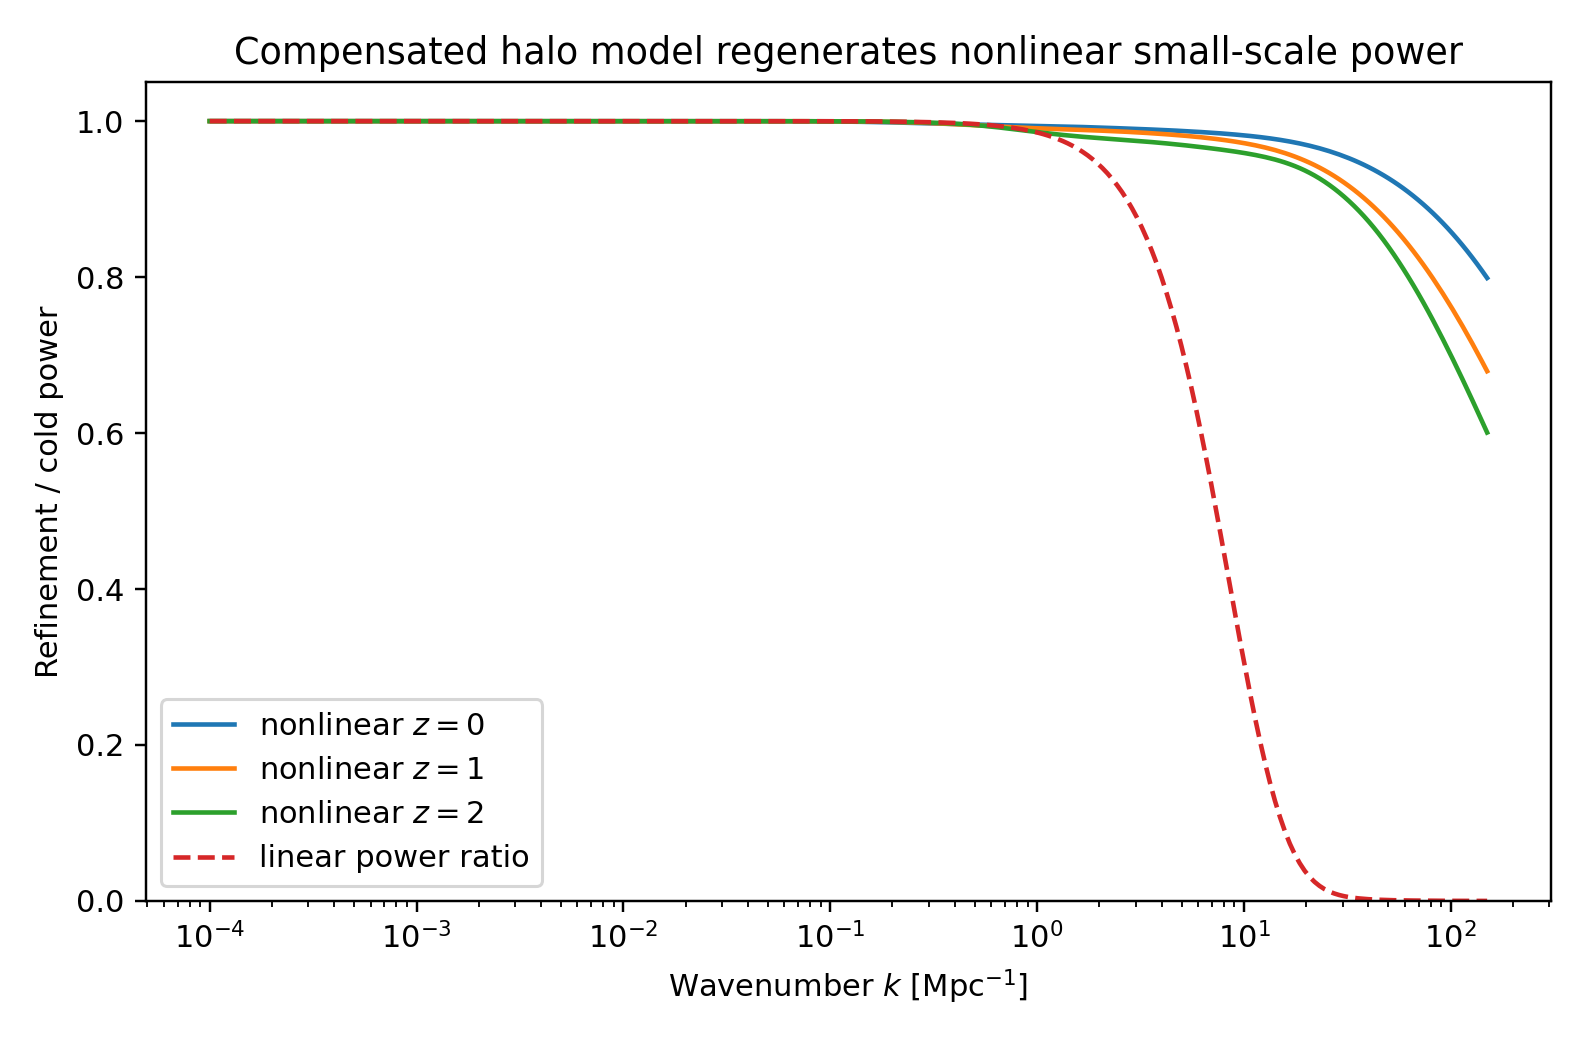
\includegraphics[width=0.88\textwidth]{figures/nls/nonlinear_power_ratios.png}
\caption{The dashed curve is the linear power ratio.  The solid curves are the compensated nonlinear halo-model ratios.  Nonlinear collapse substantially regenerates small-scale power.}
\label{fig:nlh-power}
\end{figure}

\section{Correction to the linear high-multipole lensing forecast}

Projecting the nonlinear halo-model power through a single-source lensing kernel gives the following ratios:
\begin{equation}
 \begin{array}{c|cccc}
 z_s&\ell=1000&\ell=3000&\ell=5000&\ell=10000\\
 \hline
 0.5&0.9926&0.9885&0.9850&0.9770\\
 1.0&0.9938&0.9903&0.9879&0.9826\\
 2.0&0.9953&0.9908&0.9886&0.9843.
 \end{array}
 \label{eq:nlh-nonlinear-lensing}
\end{equation}
The earlier linear calculation gave
\begin{equation}
 \frac{C_{5000,D}^{\kappa\kappa}(z_s=0.5)}
 {C_{5000,\rm c}^{\kappa\kappa}(z_s=0.5)}
 =0.7021280719.
 \label{eq:nlh-linear-lensing-old}
\end{equation}
The nonlinear template instead gives
\begin{equation}
 \boxed{
 \frac{C_{5000,D}^{\kappa\kappa,\rm nl}(z_s=0.5)}
 {C_{5000,\rm c}^{\kappa\kappa,\rm nl}(z_s=0.5)}
 =0.9850165782.
 }
 \label{eq:nlh-nonlinear-lensing-new}
\end{equation}
Therefore the strong linear high-$\ell$ suppression is superseded as a final forecast.  In this controlled halo model, nonlinear structure largely erases it.  Baryonic feedback and a calibrated nonlinear emulator remain necessary before a precision lensing claim can be made.

\begin{figure}[htbp]
\centering
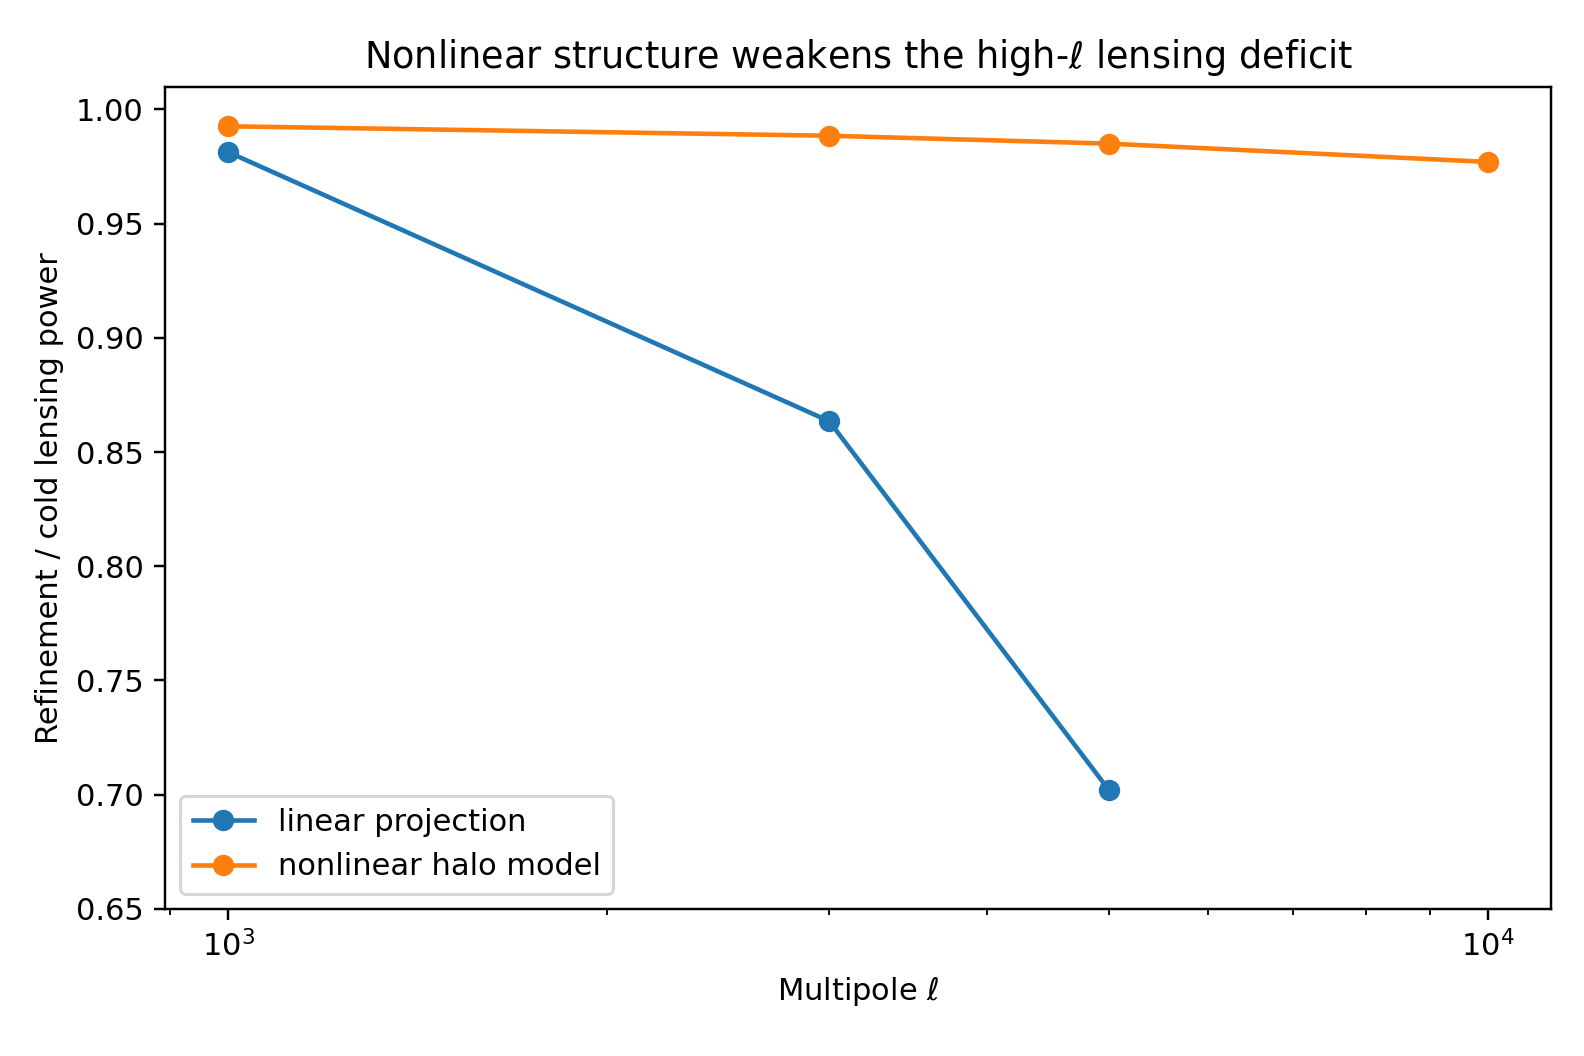
\includegraphics[width=0.84\textwidth]{figures/nls/linear_vs_nonlinear_lensing.png}
\caption{The earlier linear projection and the present nonlinear halo-model projection for $z_s=0.5$.  Nonlinear power regeneration removes most of the large linear high-$\ell$ deficit.}
\label{fig:nlh-lensing-correction}
\end{figure}

\section{Reionization consistency}

Use the declared atomic-cooling threshold
\begin{equation}
 M_{\rm atom}(z)
 =10^8M_\odot
 \left(\frac{1+z}{10}\right)^{-3/2}.
 \label{eq:nlh-atomic-mass}
\end{equation}
The collapsed fraction is
\begin{equation}
 f_{\rm coll}(>M,z)
 =\frac{1}{\bar\rho_m}
 \int_M^\infty
 M'\frac{dn}{d\log M'}\,d\log M'.
 \label{eq:nlh-collapsed-fraction}
\end{equation}
If a simple ionization model has $Q_{\rm HII}\propto\zeta_{\rm ion}f_{\rm coll}$, the same ionization history requires
\begin{equation}
 \boxed{
 \frac{\zeta_{\rm ion,D}}{\zeta_{\rm ion,c}}
 =\frac{f_{\rm coll,c}}{f_{\rm coll,D}}.
 }
 \label{eq:nlh-efficiency-penalty}
\end{equation}

The controlled results are
\begin{equation}
 \begin{array}{c|cccc}
 z&6.0&7.4&8.0&10.0\\
 \hline
 f_{\rm coll,D}/f_{\rm coll,c}
 &0.4673&0.3423&0.2944&0.1661\\
 \zeta_D/\zeta_{\rm c}
 &2.1400&2.9216&3.3973&6.0212.
 \end{array}
 \label{eq:nlh-reionization-table}
\end{equation}
At the calibrated reionization midpoint $z\simeq7.4$, the current benchmark therefore requires approximately three times the ionizing efficiency of the cold control.

\begin{figure}[htbp]
\centering
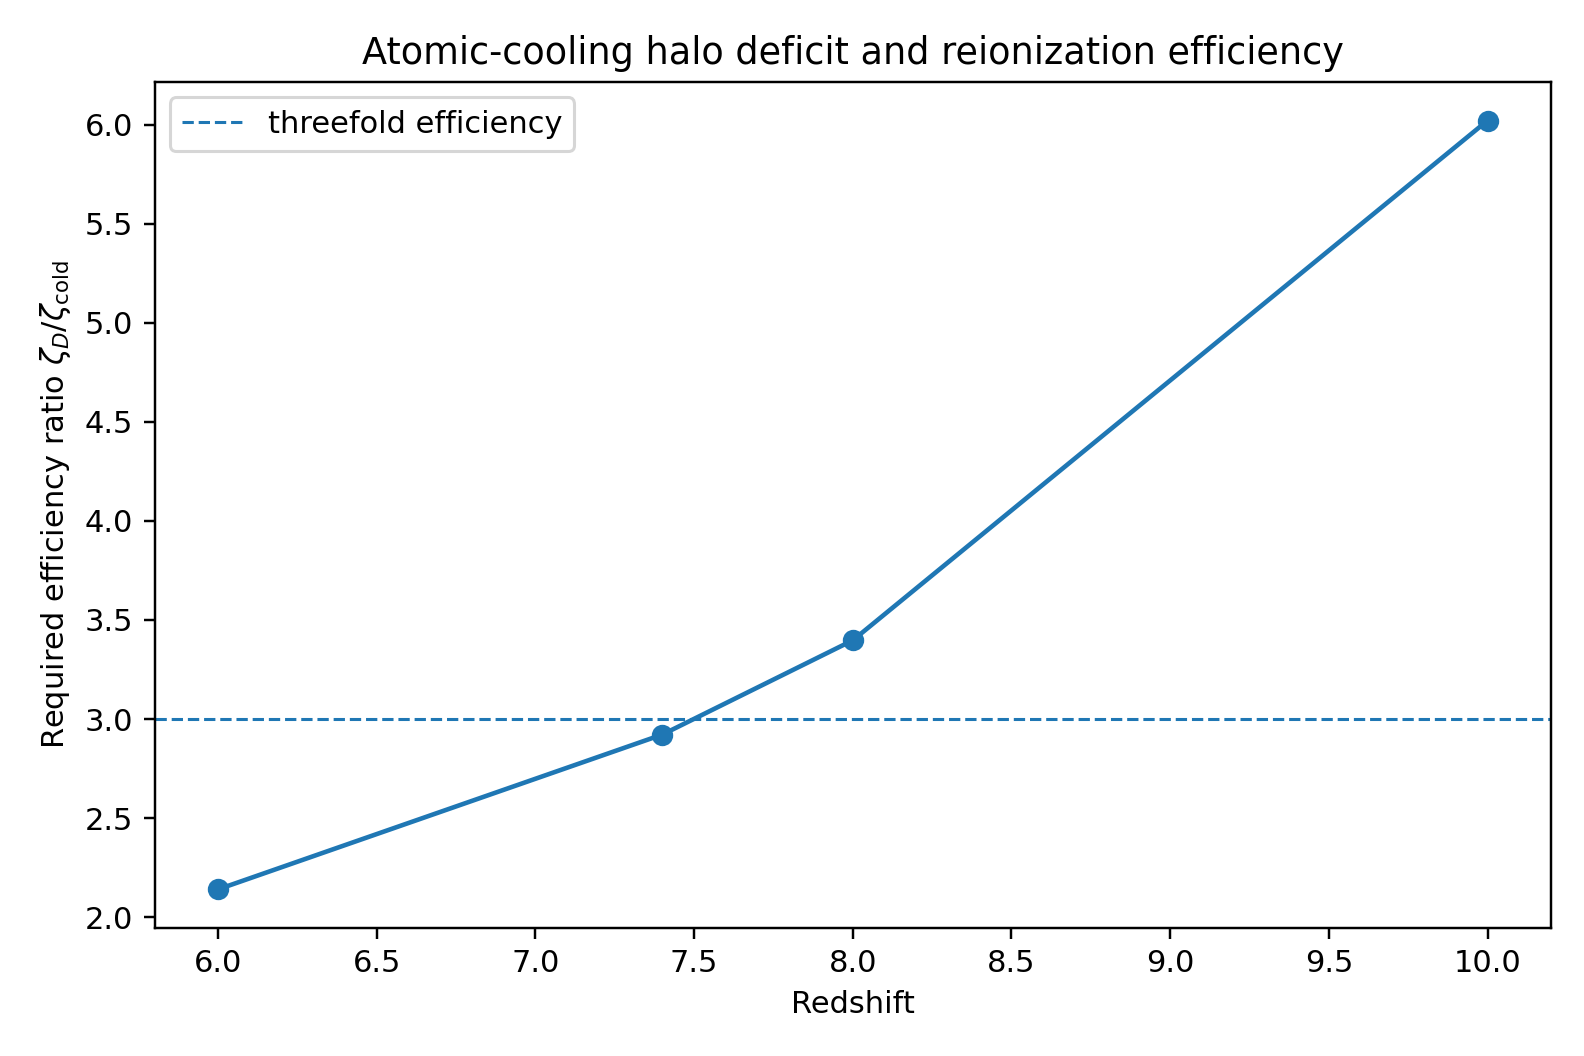
\includegraphics[width=0.82\textwidth]{figures/nls/reionization_efficiency_penalty.png}
\caption{Required ionizing-efficiency ratio in the atomic-cooling halo model.  The present cutoff produces a substantial high-redshift halo deficit.}
\label{fig:nlh-reionization}
\end{figure}

\subsection{Production-epoch bound}

The scale-covariant cutoff obeys the approximate scaling
\begin{equation}
 k_{1/2}\propto a_\star^{-1}.
 \label{eq:nlh-cutoff-scaling}
\end{equation}
Rescaling the fixed transfer while holding the remaining background inputs unchanged gives
\begin{equation}
 \begin{array}{c|cccc}
 \text{maximum efficiency penalty}
 &1.5&2&3&5\\
 \hline
 a_{\star,\max}
 &4.67\times10^{-7}
 &6.95\times10^{-7}
 &1.02\times10^{-6}
 &1.46\times10^{-6}\\
 k_{1/2,\min}\ [{\rm Mpc}^{-1}]
 &15.74&10.58&7.19&5.04.
 \end{array}
 \label{eq:nlh-production-bounds}
\end{equation}
The benchmark $a_\star=10^{-6}$ therefore lies close to the boundary of a threefold efficiency penalty.  Earlier production would move the cutoff to smaller spatial scales and ease the reionization burden.

\section{Verification}

The deterministic audit records
\begin{equation}
 \boxed{
 24\ {\rm PASS},
 \qquad
 0\ {\rm FAIL}.
 }
 \label{eq:nlh-pass-count}
\end{equation}
Selected controls are
\begin{equation}
 \begin{array}{c|c}
 \text{control}&\text{residual or discrepancy}\\
 \hline
 \sigma_8\ \text{reconstruction}&0\\
 T_D(k_{1/2})^2-1/2&1.11\times10^{-16}\\
 \text{one-halo low-}k\text{ slope error}&2.13\times10^{-3}\\
 \text{mass-grid refinement}&3.31\times10^{-5}\\
 \text{lensing-grid refinement}&2.89\times10^{-6}.
 \end{array}
 \label{eq:nlh-verification-table}
\end{equation}

\section{Claim boundary and resulting direction}

This chapter is a controlled semi-analytic nonlinear closure.  It does not establish:
\begin{itemize}
 \item a first-principles halo mass function from the projector action;
 \item calibrated halo concentrations or subhalo disruption;
 \item hydrodynamics, star formation, feedback, or metal enrichment;
 \item nonlinear Vlasov evolution from the production surface;
 \item a precision nonlinear matter emulator;
 \item a galaxy survey, reionization, or lensing likelihood;
 \item observational correctness or literature priority.
\end{itemize}

The robust result is not the exact numerical value of the halo-model lensing ratio.  It is the separation
\begin{equation}
 \boxed{
 \begin{aligned}
 \text{linear and high-redshift statistics}
 &:\ \text{strong cutoff sensitivity},\\
 \text{deeply nonlinear projected power}
 &:\ \text{substantial gravitational regeneration}.
 \end{aligned}}
 \label{eq:nlh-observable-separation}
\end{equation}
A full nonlinear test therefore requires a particle or phase-space solver with baryonic source terms, followed by a frozen-parameter likelihood using the low-mass halo abundance, reionization history, CMB lensing, and galaxy lensing together.
